\documentclass[14pt]{extbook}
\usepackage{multicol, enumerate, enumitem, hyperref, color, soul, setspace, parskip, fancyhdr} %General Packages
\usepackage{amssymb, amsthm, amsmath, latexsym, units, mathtools} %Math Packages
\everymath{\displaystyle} %All math in Display Style
% Packages with additional options
\usepackage[headsep=0.5cm,headheight=12pt, left=1 in,right= 1 in,top= 1 in,bottom= 1 in]{geometry}
\usepackage[usenames,dvipsnames]{xcolor}
\usepackage{dashrule}  % Package to use the command below to create lines between items
\newcommand{\litem}[1]{\item#1\hspace*{-1cm}\rule{\textwidth}{0.4pt}}
\pagestyle{fancy}
\lhead{Progress Quiz 5}
\chead{}
\rhead{Version C}
\lfoot{8497-6012}
\cfoot{}
\rfoot{Summer C 2021}
\begin{document}

\begin{enumerate}
\litem{
Solve the radical equation below. Then, choose the interval(s) that the solution(s) belongs to.\[ \sqrt{5 x + 3} - \sqrt{-4 x + 4} = 0 \]\begin{enumerate}[label=\Alph*.]
\item \( x_1 \in [-0.76, -0.54] \text{ and } x_2 \in [-0.48,0.56] \)
\item \( x_1 \in [-0.76, -0.54] \text{ and } x_2 \in [0.51,1.27] \)
\item \( x \in [-1.03,-0.63] \)
\item \( x \in [0.03,0.38] \)
\item \( \text{All solutions lead to invalid or complex values in the equation.} \)

\end{enumerate} }
\litem{
Choose the graph of the equation below.\[ f(x) = - \sqrt[3]{x + 10} - 4 \]\begin{enumerate}[label=\Alph*.]
\begin{multicols}{2}\item 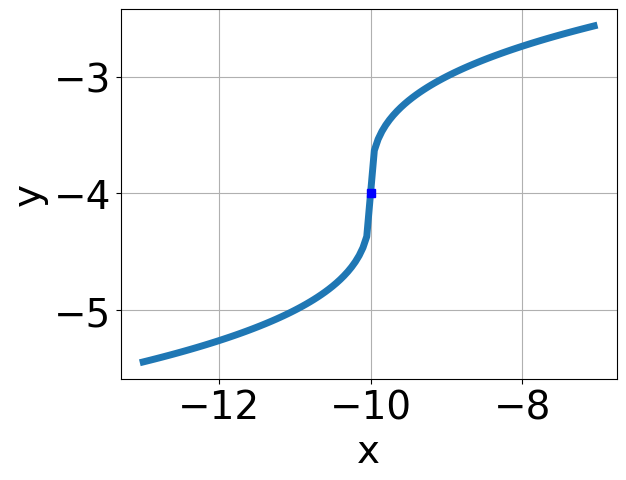
\includegraphics[width = 0.3\textwidth]{../Figures/radicalEquationToGraphCopyAC.png}\item 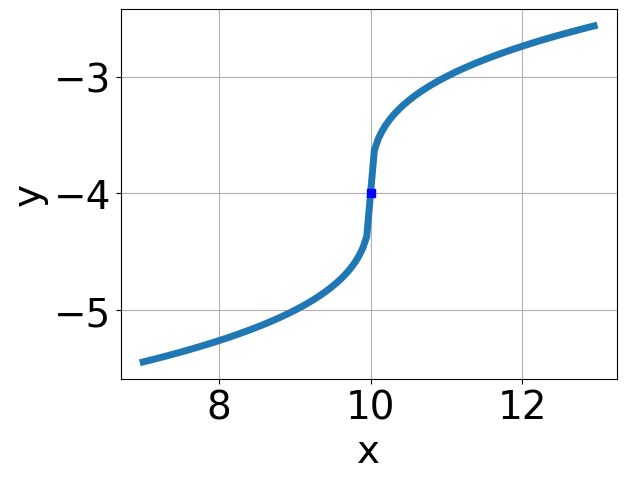
\includegraphics[width = 0.3\textwidth]{../Figures/radicalEquationToGraphCopyBC.png}\item 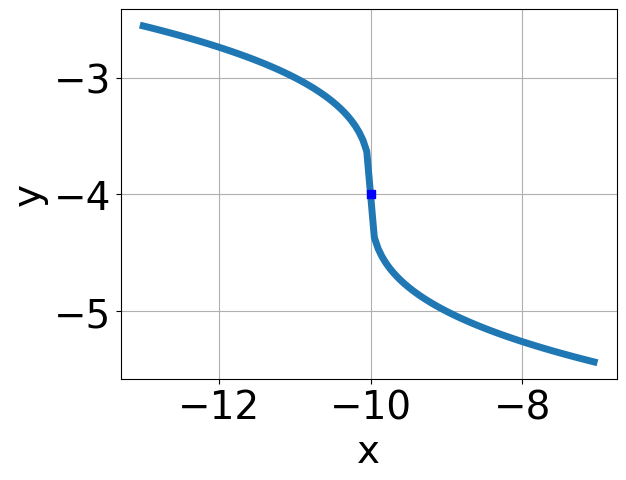
\includegraphics[width = 0.3\textwidth]{../Figures/radicalEquationToGraphCopyCC.png}\item 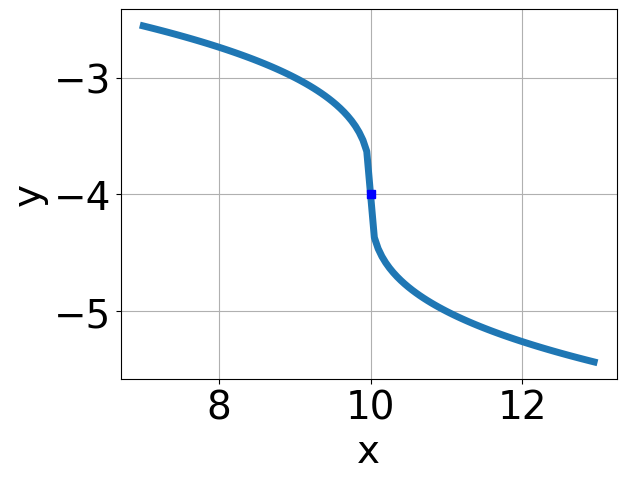
\includegraphics[width = 0.3\textwidth]{../Figures/radicalEquationToGraphCopyDC.png}\end{multicols}\item None of the above.
\end{enumerate} }
\litem{
Choose the equation of the function graphed below.
\begin{center}
    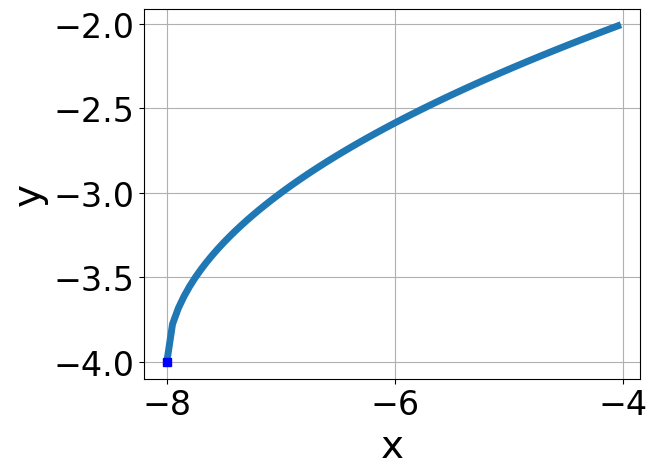
\includegraphics[width=0.5\textwidth]{../Figures/radicalGraphToEquationC.png}
\end{center}
\begin{enumerate}[label=\Alph*.]
\item \( f(x) = - \sqrt{x - 8} - 4 \)
\item \( f(x) = \sqrt{x + 8} - 4 \)
\item \( f(x) = - \sqrt{x + 8} - 4 \)
\item \( f(x) = \sqrt{x - 8} - 4 \)
\item \( \text{None of the above} \)

\end{enumerate} }
\litem{
Solve the radical equation below. Then, choose the interval(s) that the solution(s) belongs to.\[ \sqrt{-16 x^2 + 36} - \sqrt{-14 x} = 0 \]\begin{enumerate}[label=\Alph*.]
\item \( x \in [1.9,2.8] \)
\item \( x_1 \in [-1.23, -0.78] \text{ and } x_2 \in [-1,3] \)
\item \( x \in [-1.23,-0.78] \)
\item \( \text{All solutions lead to invalid or complex values in the equation.} \)
\item \( x_1 \in [1.05, 1.16] \text{ and } x_2 \in [-1,3] \)

\end{enumerate} }
\litem{
Solve the radical equation below. Then, choose the interval(s) that the solution(s) belongs to.\[ \sqrt{6 x - 2} - \sqrt{-7 x + 9} = 0 \]\begin{enumerate}[label=\Alph*.]
\item \( \text{All solutions lead to invalid or complex values in the equation.} \)
\item \( x \in [0.38,1.4] \)
\item \( x_1 \in [-0.07, 0.7] \text{ and } x_2 \in [1,1.4] \)
\item \( x \in [-1.36,-0.06] \)
\item \( x_1 \in [-0.07, 0.7] \text{ and } x_2 \in [0.8,1] \)

\end{enumerate} }
\litem{
What is the domain of the function below?\[ f(x) = \sqrt[7]{-7 x - 9} \]\begin{enumerate}[label=\Alph*.]
\item \( \text{The domain is } [a, \infty), \text{   where } a \in [-0.81, 0.1] \)
\item \( (-\infty, \infty) \)
\item \( \text{The domain is } (-\infty, a], \text{   where } a \in [-1.24, 0.46] \)
\item \( \text{The domain is } (-\infty, a], \text{   where } a \in [-1.4, -0.78] \)
\item \( \text{The domain is } [a, \infty), \text{   where } a \in [-1.49, -1.01] \)

\end{enumerate} }
\litem{
Choose the graph of the equation below.\[ f(x) = - \sqrt[3]{x + 8} - 3 \]\begin{enumerate}[label=\Alph*.]
\begin{multicols}{2}\item 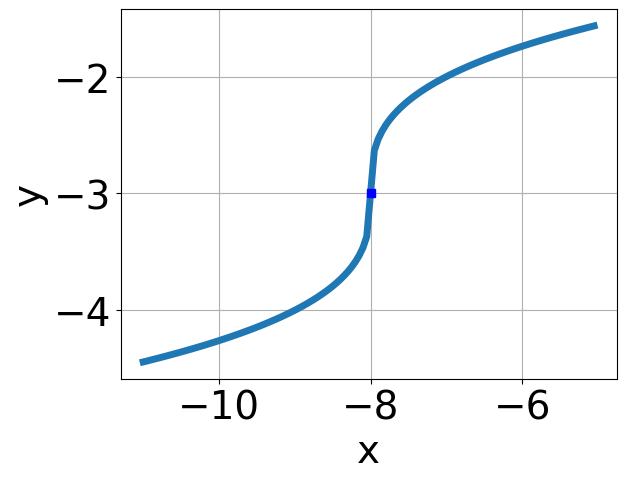
\includegraphics[width = 0.3\textwidth]{../Figures/radicalEquationToGraphAC.png}\item 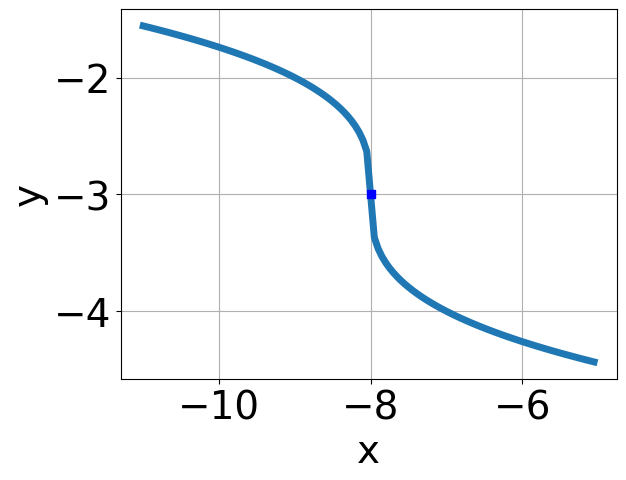
\includegraphics[width = 0.3\textwidth]{../Figures/radicalEquationToGraphBC.png}\item 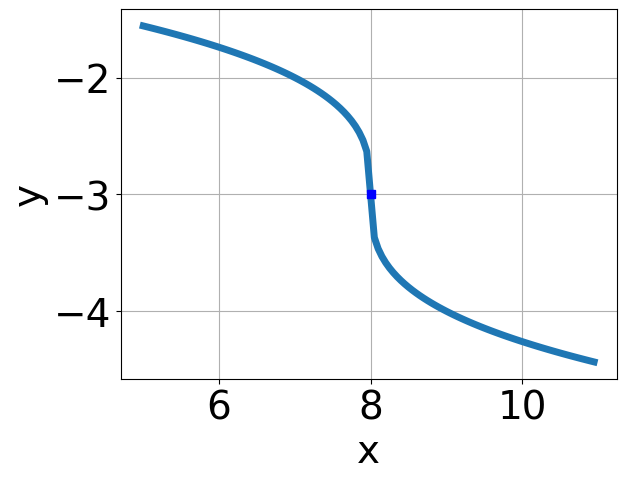
\includegraphics[width = 0.3\textwidth]{../Figures/radicalEquationToGraphCC.png}\item 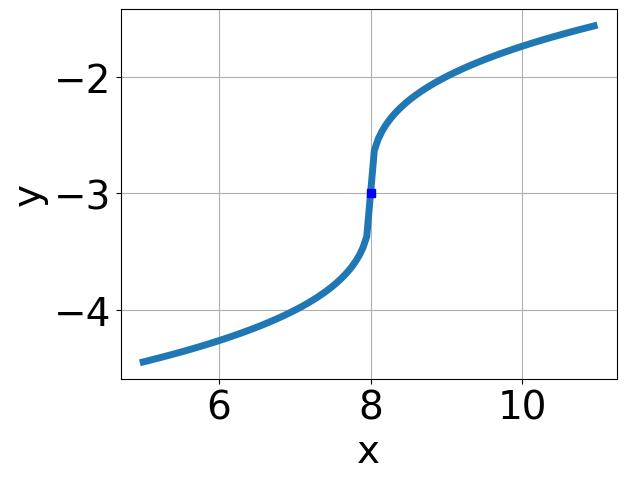
\includegraphics[width = 0.3\textwidth]{../Figures/radicalEquationToGraphDC.png}\end{multicols}\item None of the above.
\end{enumerate} }
\litem{
Choose the equation of the function graphed below.
\begin{center}
    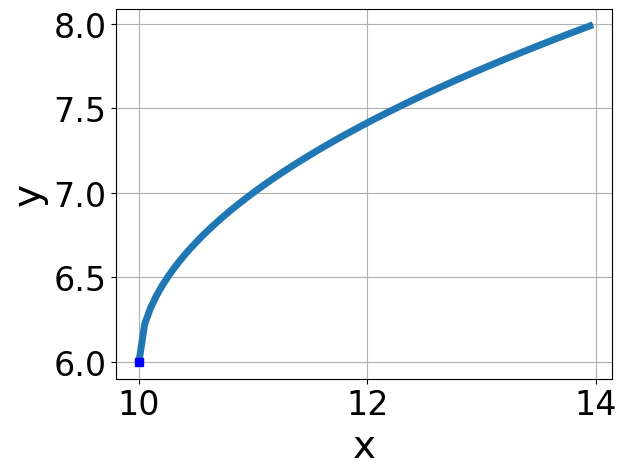
\includegraphics[width=0.5\textwidth]{../Figures/radicalGraphToEquationCopyC.png}
\end{center}
\begin{enumerate}[label=\Alph*.]
\item \( f(x) = - \sqrt[3]{x - 10} + 6 \)
\item \( f(x) = \sqrt[3]{x + 10} + 6 \)
\item \( f(x) = \sqrt[3]{x - 10} + 6 \)
\item \( f(x) = - \sqrt[3]{x + 10} + 6 \)
\item \( \text{None of the above} \)

\end{enumerate} }
\litem{
Solve the radical equation below. Then, choose the interval(s) that the solution(s) belongs to.\[ \sqrt{40 x^2 + 42} - \sqrt{-83 x} = 0 \]\begin{enumerate}[label=\Alph*.]
\item \( \text{All solutions lead to invalid or complex values in the equation.} \)
\item \( x \in [-1.17,-0.73] \)
\item \( x_1 \in [0.82, 1.04] \text{ and } x_2 \in [-0.8,3.2] \)
\item \( x \in [-1.78,-1.01] \)
\item \( x_1 \in [-1.78, -1.01] \text{ and } x_2 \in [-1.87,1.13] \)

\end{enumerate} }
\litem{
What is the domain of the function below?\[ f(x) = \sqrt[6]{-4 x + 5} \]\begin{enumerate}[label=\Alph*.]
\item \( (-\infty, \infty) \)
\item \( (-\infty, a], \text{ where } a \in [0.82, 1.31] \)
\item \( (-\infty, a], \text{where } a \in [0.55, 0.93] \)
\item \( [a, \infty), \text{where } a \in [0.59, 1.19] \)
\item \( [a, \infty), \text{where } a \in [1.1, 1.43] \)

\end{enumerate} }
\end{enumerate}

\end{document}